As demonstrated in recent research by Farzan Majeed Noori,
Benedikte Wallace, Md. Zia Uddin and Jim Torresen in \cite{10.1007/978-3-030-20205-7_25}, a combined architecture of using OpenPose for pose estimation and Recurrent Neural Networks (RNN) for human activity recognition could prove as the new state-of-the-art solution for robust and non-intrusive human activity recognition. In the cited research, OpenPose was used to extract keypoints from a subset of the Berkeley Multimodal Human Action Database (BMHAD) \cite{Berkeley-MHAD}. What makes it remarkable is the classification accuracy obtained using a Recurrent Neural Network with Long Short-term Memory (LSTM) cells over more conventional machine learning classifiers, such as Support Vector Machines, Decision Trees and Random Forests. Since the dataset contained human activities recorded from different angles, the solution is also view-invariant, increasing the robustness of this solution. Another paper, a technical report by Chinmay Sawant \cite{sawant2020human}, also supports the combination of OpenPose with LSTMs for time-series classification, reporting similar accuracy results in a real-time application on the same BMHAD dataset, making use of the efficiency of this solution.

The difference between the cited work and current work is the custom dataset constructed for gymnastics based movements. In contrast to the BMHAD dataset, which includes 11 general activities, such as jumping jacks, waving, and clapping, the dataset used in the current thesis uses more complex biomechanical activities, including human body rotations and airtime, such as backflips and back-handsprings. The author of this paper expects the RNNs used for general action recognition also to be applicable to gymnastics movements. This research aims to validate this hypothesis and investigate neural network architectures most suitable for gymnastics action recognition. 

\section{Methodology}

A combination of empirical knowledge with the mathematical theory of artificial neural networks is used as the starting point to develop neural networks capable of recognizing gymnastics movements. The development process starts by training a simple recurrent neural network with gymnastics data and analyzing the results. Simple RNN is chosen primarily for its known property of representing information from context window \cite{DBLP:journals/corr/Lipton15}. RNNs have \textit{long-term memory} in the form of weights, enabling the network to \textit{remember} a gymnastics element represented as a sequence. An iterative process is used to train, validate, analyze, and compare each classifier's results. The steps followed in the current thesis are represented in figure \ref{classifier-tasks}.

\begin{figure}[htb]
  \centering
    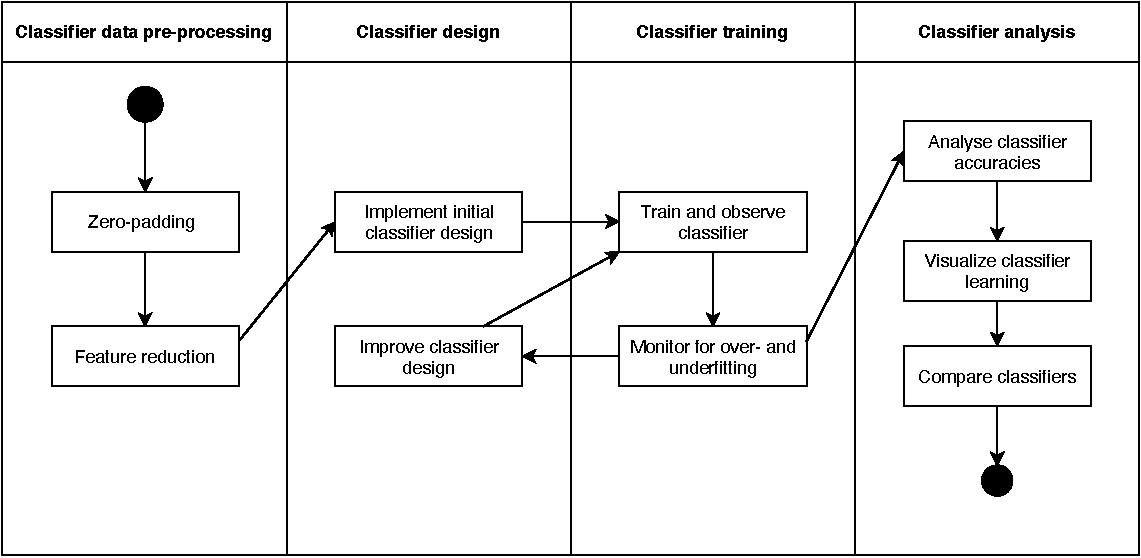
\includegraphics[width=\textwidth,keepaspectratio]
    {images/classifier/classifier-tasks}
    \caption{Tasks completed regarding classifier development in the thesis}
    \label{classifier-tasks}
\end{figure}

\subsection{Classifier Prerequisites}

Two prerequisites before feeding training data to the classifiers include:

\begin{easylist}[itemize]

& \textit{Zero-padding} --- Gymnastics activities performed vary in their length, and the samples are zero-padded to keep the classifier dimensions static. Zero-padding is done by finding the longest sample performed and increasing the timesteps of other samples with zero values until they are equal in length to the longest sample.
& \textit{Feature reduction} --- Recurrent neural networks are prone to overfitting \cite{DBLP:journals/corr/ZarembaSV14}. With the combination of the author's domain knowledge about gymnastics, the 25 total keypoints obtained during pose estimation are reduced to 15, filtering out less prominent keypoints necessary to recognize gymnastics movements. The 15 keypoints used for classification include the trunk, head, and limbs of the skeleton.

\end{easylist}

\subsection{Classifier Algorithms}

Classifier algorithms experimented with in the thesis are:

\begin{easylist}[itemize]

& \textit{Simple RNN} --- The first classifier (shown in figure \ref{simple-rnn-network-layers}) experimented with is a network model with one simple recurrent layer. The recurrent layer consists of 2 units, chosen according to the number of outputs the network produces - the movements are either a backflip or a back handspring. A dropout layer with a 0.5 rate to prevent overfitting is added next. An activation layer with rectified linear units follows with a flattening layer to reduce dimensions, and finally, an output layer with softmax activation is used for representing the different activities. Categorical cross-entropy is used as the loss function during stochastic gradient descent with an Adam optimizer with a learning rate of 0.001.
& \textit{Hierarchical RNN} --- The Simple RNN works well for the short duration activities analyzed in this paper, but the downside of using one recurrent layer is observability. By feeding all available dimensions into one recurrent layer, we lose the visibility of what exactly the different units in a neural network learn. A more advanced and deeper neural network (inspired by article \cite{hierarchical-rnn-har}) consists of several recurrent layers, each representing some logical unit. The model used for experimentation in this paper is shown in figure \ref{hierarchical-rnn-network-layers}. Hierarchical RNN uses multiple input units, each representing a human skeleton subsection. In this example, the skeleton is divided into the left arm, right arm, trunk, left leg, and right leg subsections. In subsequent layers, the recurrent units are fused, and finally, neural activations are applied on a fully connected skeleton layer. One of the advantages of this method is that we can now intercept some layer of interest and observe the neuron activations only regarding a skeleton's subsection.
& \textit{LSTM} --- An RNN with LSTM cells was also implemented. The simple recurrent layer is substituted with a hidden LSTM layer with two hidden units, accordingly representing the network's outputs. Other layers remain identical with the \textit{Simple RNN} classifier.

\end{easylist}

\begin{figure}[htb]
  \centering
    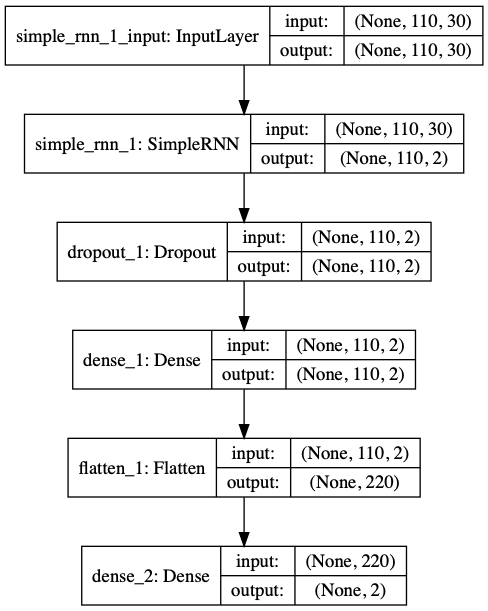
\includegraphics[width=0.7\textwidth,keepaspectratio]
    {images/classifier/simple-rnn-network-layers}
    \caption{The neural network design with a simple recurrent layer}
    \label{simple-rnn-network-layers}
\end{figure}

\begin{figure}[htb]
  \centering
    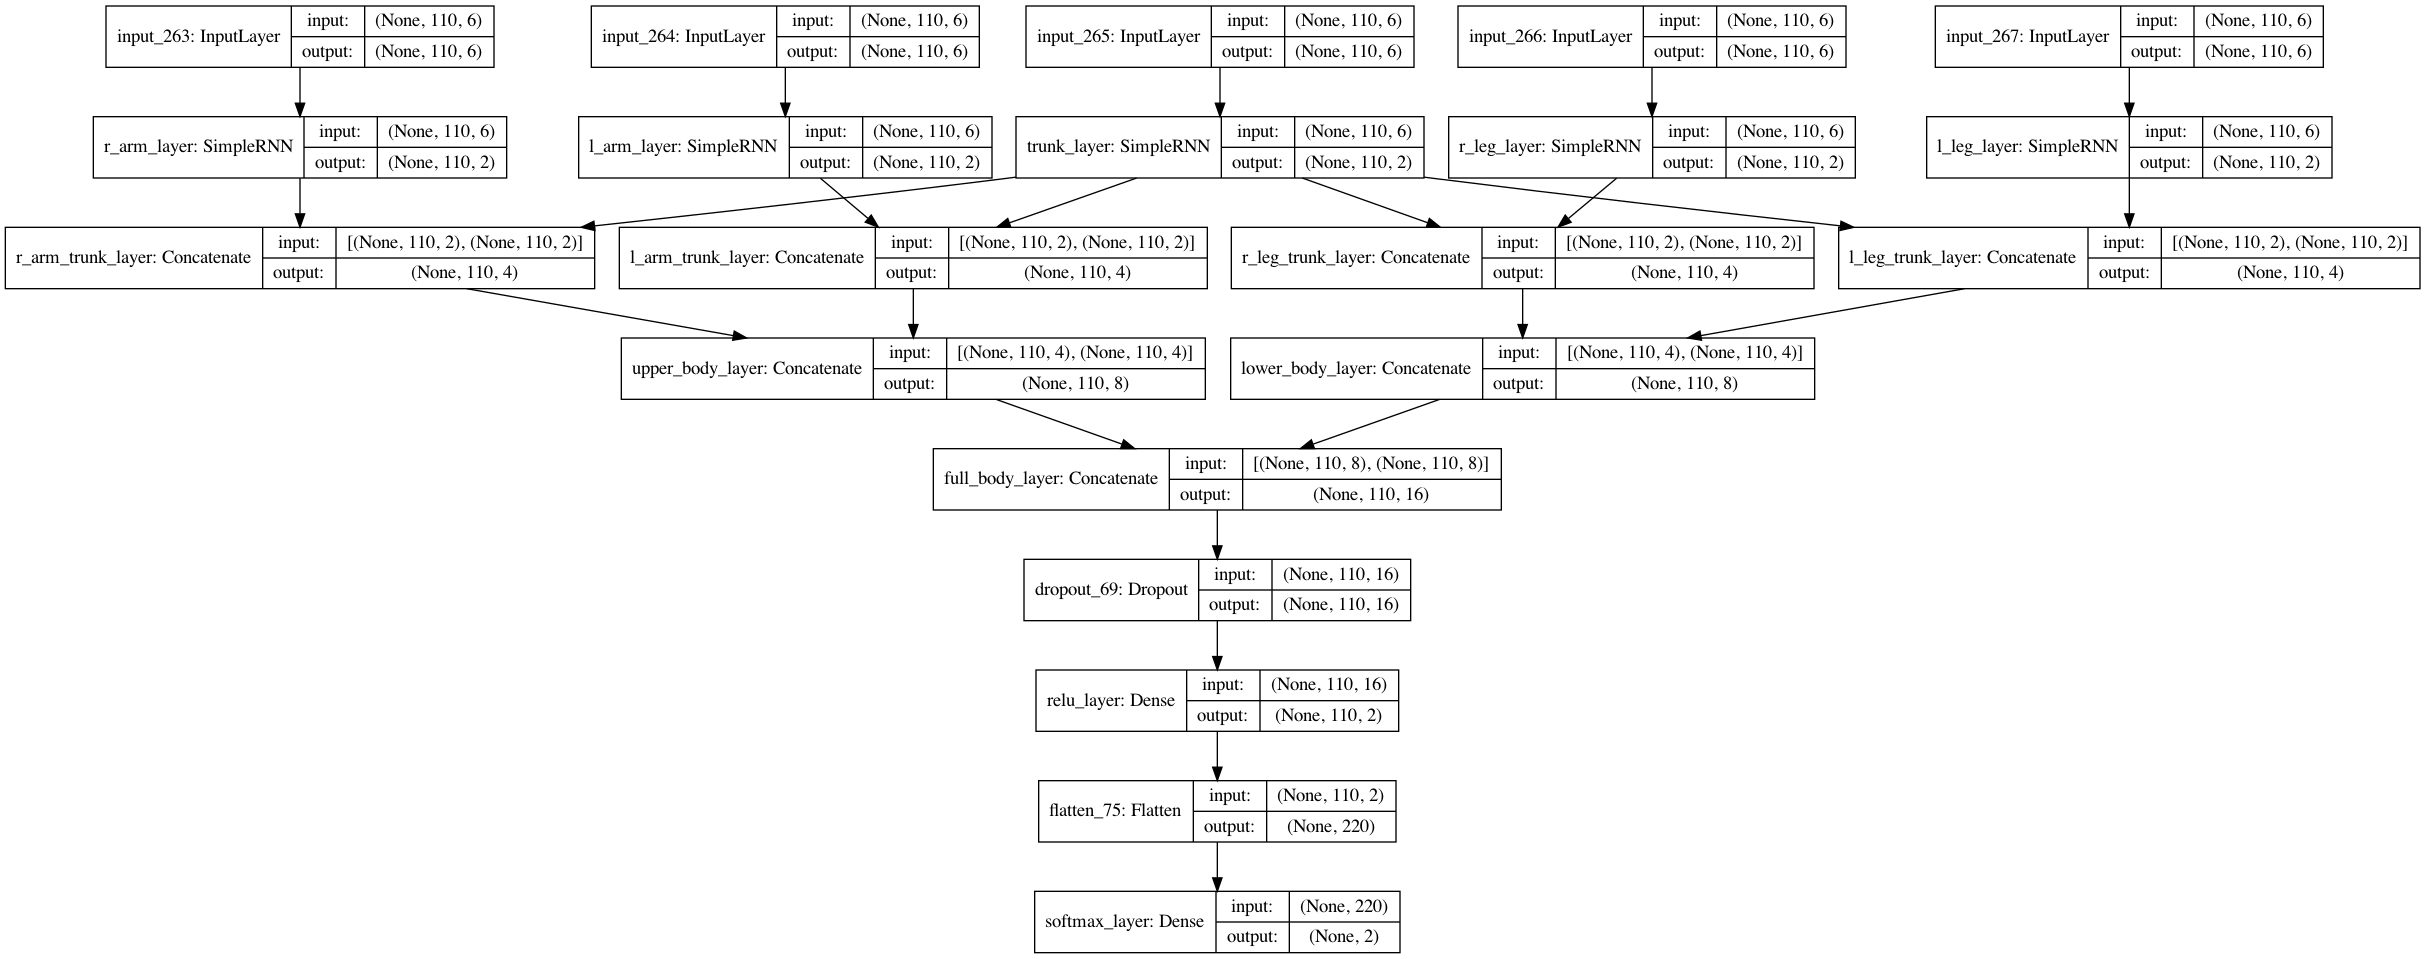
\includegraphics[width=\textwidth,keepaspectratio]
    {images/classifier/hierarchical-rnn-model-summary}
    \caption{The neural network design with hierarchical recurrent layers}
    \label{hierarchical-rnn-network-layers}
\end{figure}

\subsection{Classifier Validation}

Validating the learning process of our neural networks requires the usage of some standard classifier validation techniques. First, we list these validation methods for reference and then explain each one more thoroughly: 

\begin{easylist}[itemize]

& \textit{Test split} --- 0.2 rates split the sample data between training and testing data to test for unbiased results when the model training has stopped.
& \textit{Validation split} --- A validation split of 0.33 rate is also used while training the RNN to observe the model's loss and accuracy, essential to help with hyperparameter tuning. The validation set is kept separately from the test set, so when we optimize our hyperparameters, we can validate our results against the test set.
& \textit{Monitoring accuracy and loss} --- Figure \ref{model-validation-monitoring} demonstrates how the LSTM model accuracy and loss are monitored during epochs to detect overfitting or underfitting. When the training and test set accuracies and losses do not diverge too much, we can be more confident that our classifier is generalizing and not just optimizing for the input data \cite{deep-learning-cookbook}.
& \textit{Repeated training on unconnected models} --- We repeat each classifier training on five unconnected models. As stated in \cite{bianchini1994problem}, the optimization of a cost function in recurrent neural networks can potentially lead some minima that are not the most optimal (global). By running our experiment on five unconnected models, we avoid basing our observations and analysis under the influence of one sub-optimal (local) minima.
& \textit{Recurrent neural network regularization} --- As we train a deep neural network on a small training set, we experience what is known as the "overfitting" phenomenon, observed when training the classifiers, and achieving a test accuracy of 100\%. In our case, this happens due to repeated training on a small dataset with little variance. We add dropout layers to randomly omit half of the feature detectors on each training case \cite{hinton2012improving}.

\end{easylist}

\begin{figure*}
   \centering
\begin{tabular}{cc}
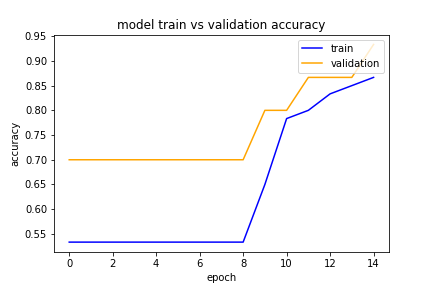
\includegraphics[width=7.5cm]{images/classifier/model-train-vs-validation-accuracy}&
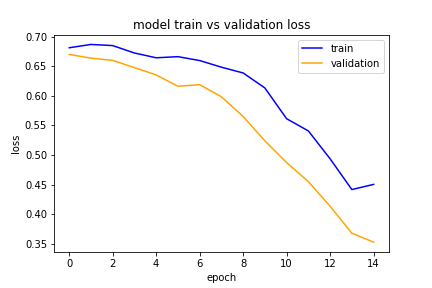
\includegraphics[width=7.5cm]{images/classifier/model-train-vs-validation-loss}\\
\end{tabular}
    \caption{Monitoring for model accuracy and loss to detect overfitting/underfitting}
    \label{model-validation-monitoring}
\end{figure*}

\subsection{Classifier Training Process}
\label{classifier-training-process}

\subsubsection{Simple RNN} 

Due to the small sample data size, the RNN classifier is trained for 5 epochs with stochastic gradient descent. The hyperparameters are empirically selected for the classifier, with the goal to maximize the accuracy while preventing overfitting.

An early stopping hook (callback) is also implemented to monitor for validation loss improvements. No improvements in validation loss commonly indicate that the network has stopped learning and is starting to overfit to the training data. After 3 epochs with no improvements the hook stops the learning process of the neural network. 

\begin{figure*}
    \centering
\begin{tabular}{c|c}
    \bfseries Repeat & \bfseries Accuracy (\%) % specify table head
    \csvreader[head to column names]{simple-rnn-repeats-accuracy.csv}{} % use head of csv as column names
    {\\\hline\i & \a} % specify your coloumns here
\end{tabular}
    \caption{Mean accuracies obtained during each Simple RNN classifier run}
    \label{simple-rnn-repeats-accuracy}
\end{figure*}

\section{Classifier Visualization and Analysis}
\label{classifier-visualization}

\subsubsection{Simple RNN} 

The fourth experiment run (from table \ref{simple-rnn-repeats-accuracy}) is chosen to dive deeper into the inner workings of the classifier.

By configuring the model's RNN layer to return hidden states, it is possible to intercept the output values of this layer and investigate the neuron activations. It is also possible to visualize these activations to better understand what the neurons are learning. The neuron visualization code is based on the code found in \textit{Deep Learning Cookbook} by Douwe Osinga \cite{deep-learning-cookbook}, but with a major difference in the data being used as the input for the recurrent network. In section \textit{5.5 Visualizing Recurrent Network Activations}, Douwe Osinga uses a bitmap to visualize a \textbf{text sequence} being provided to the network and intercepting the activations of a specific layer. However, the current work uses \textbf{time-series data} representing skeleton keypoints location for each frame of a gymnastics activity. This requires some modifications to the visualization code provided in the book. The modified code snippet is added as an appendix (\ref{visualizing-recurrent-network-appendix}) to this thesis, as to the best of author's knowledge, there are not many examples of recurrent neural network neuron activation visualization code for time-series skeleton data available.

The author of this work compares neuron activations of backflips (figure \ref{backflip-neuron-activations-simple-rnn}) and back handsprings (figure \ref{back-handspring-neuron-activations-simple-rnn}). In both figures, the activations are visualized using four horizontal lines. Each horizontal line also consists of three inner lines, where the first represents timestep indices and other two represent activations of two hidden layer neurons. The outer horizontal lines are split by 30 timesteps, which correspond to 0.5 seconds of activity time since the activities are recorded at 60 frames per second.

As a reminder, all samples are 110 timesteps long and the missing values are zero-padded. The chosen samples are also correctly predicted by the model. It is interesting to observe how the first neuron starts to flicker it's activation when it encounters the ending of an activity. From here we can also observe how back handsprings tend to last longer than backflips, easily noticeable from neuron activations. A second observation can be made by noticing that the first neuron seems to activate throughout almost the whole duration of a backflip. 

\begin{figure*}
   \centering
\begin{tabular}{c}
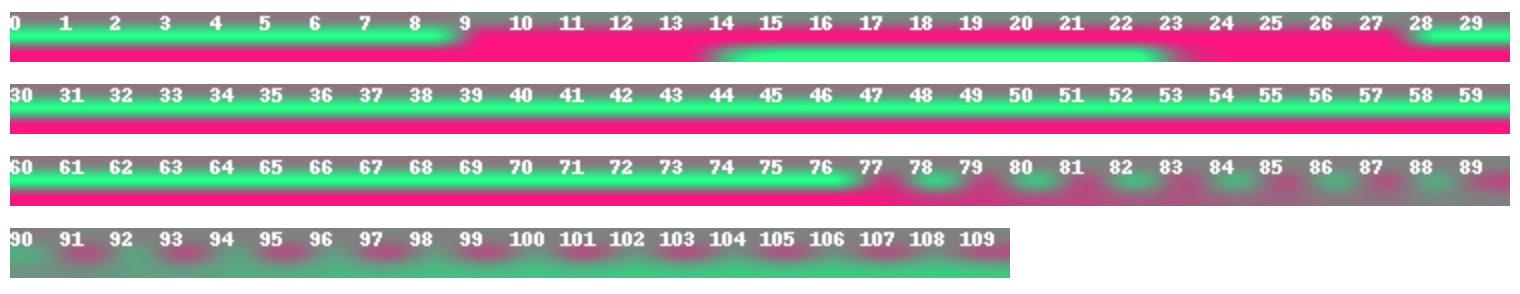
\includegraphics[width=\textwidth]{images/classifier/neuron-activations-simple-rnn-model-3/backflip-23-tiit}\\
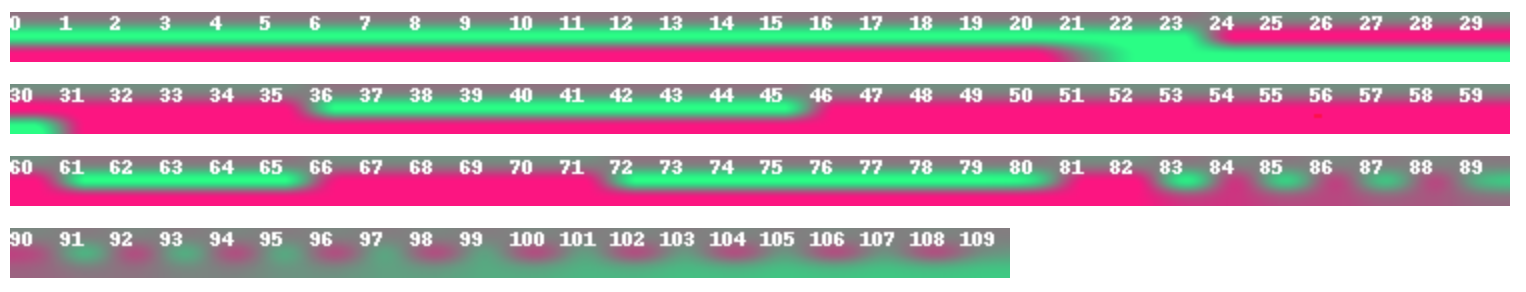
\includegraphics[width=\textwidth]{images/classifier/neuron-activations-simple-rnn-model-3/backflip-40-margus}\\
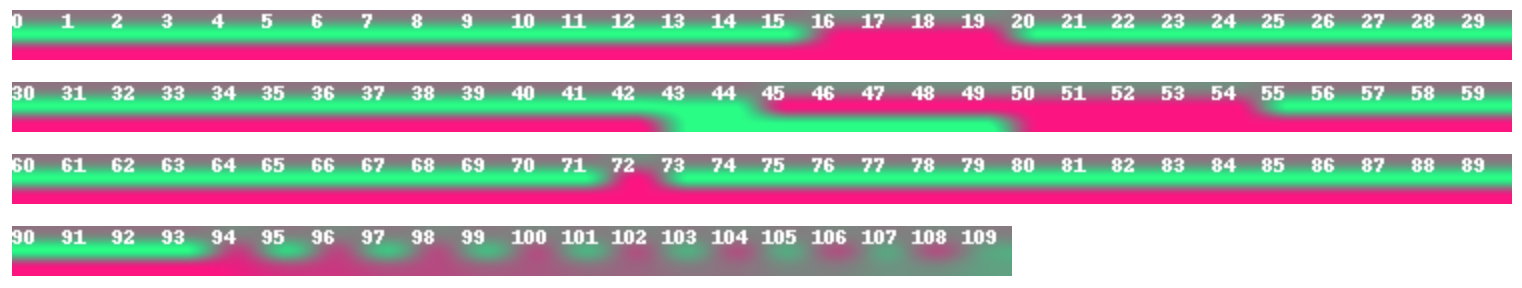
\includegraphics[width=\textwidth]{images/classifier/neuron-activations-simple-rnn-model-3/backflip-6-rasmus}\\
%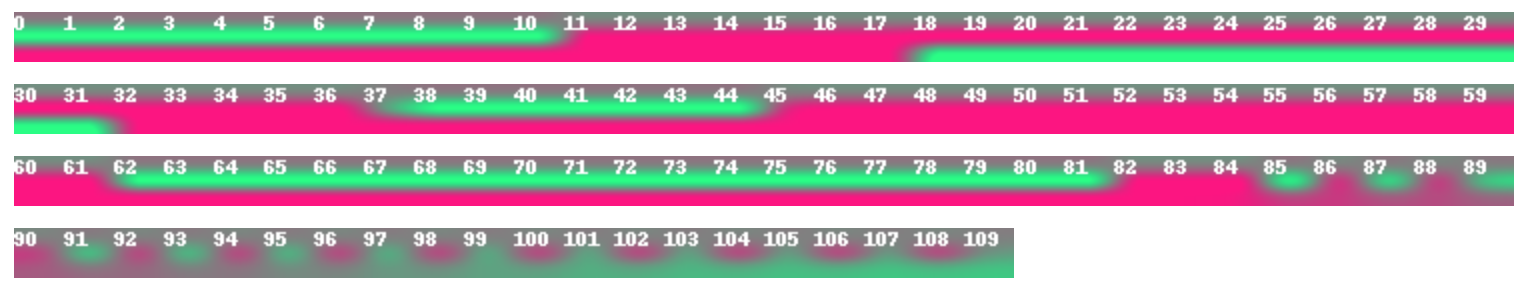
\includegraphics[width=\textwidth]{images/classifier/neuron-activations-simple-rnn-model-3/backflip-64-allar}\\
%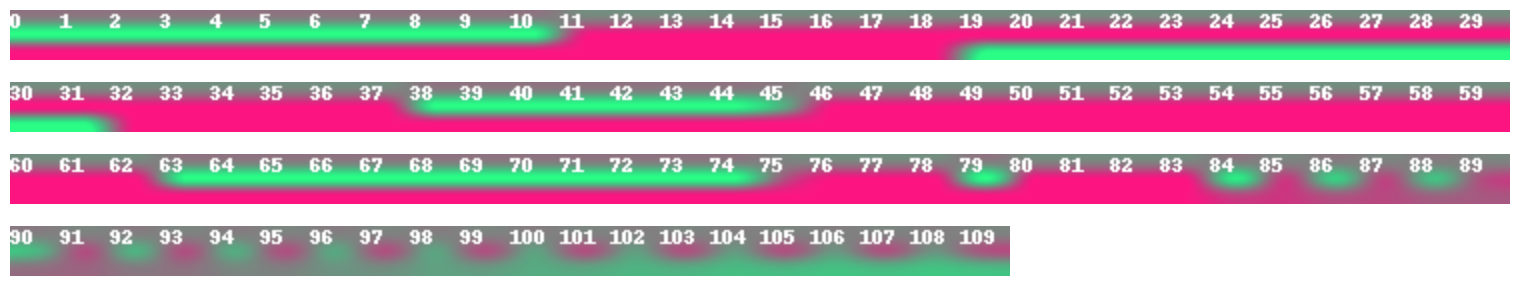
\includegraphics[width=\textwidth]{images/classifier/neuron-activations-simple-rnn-model-3/backflip-66-allar}\\
\end{tabular}
    \caption{Simple RNN neuron activations for backflip samples}
    \label{backflip-neuron-activations-simple-rnn}
\end{figure*}

\begin{figure*}
   \centering
\begin{tabular}{c}
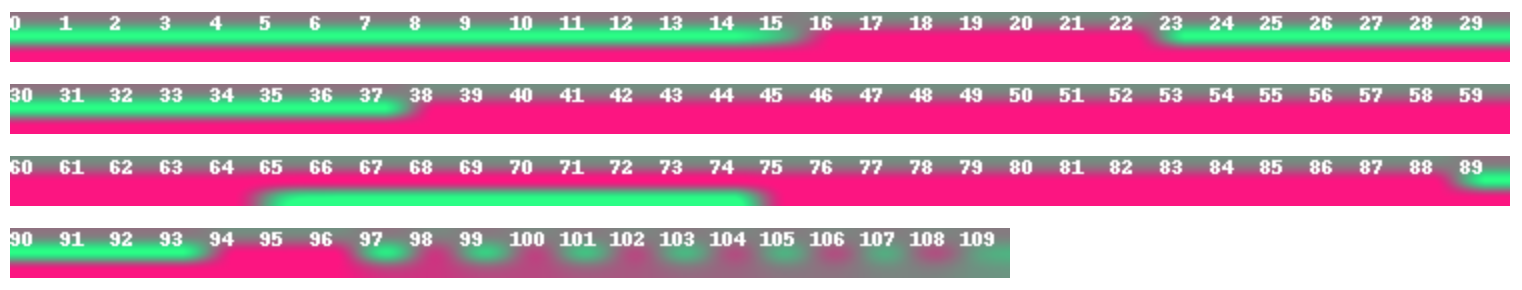
\includegraphics[width=\textwidth]{images/classifier/neuron-activations-simple-rnn-model-3/flack-19-rasmus}\\
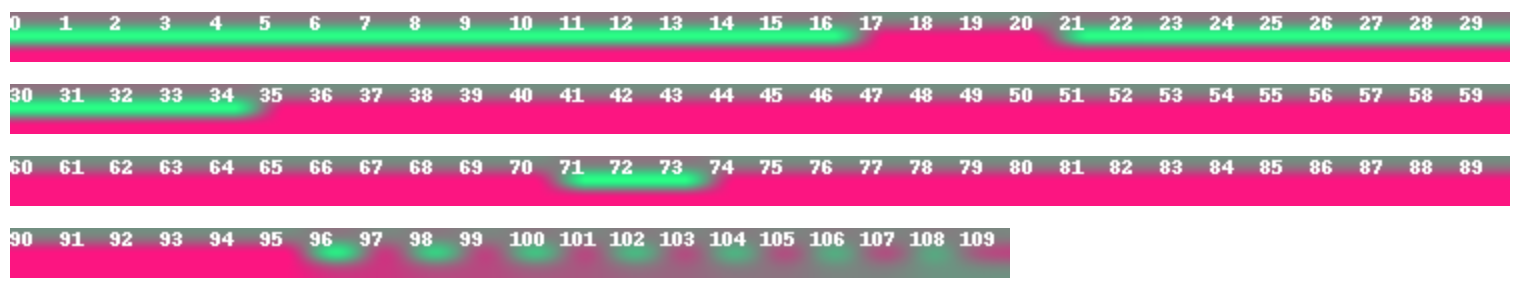
\includegraphics[width=\textwidth]{images/classifier/neuron-activations-simple-rnn-model-3/flack-31-rasmus}\\
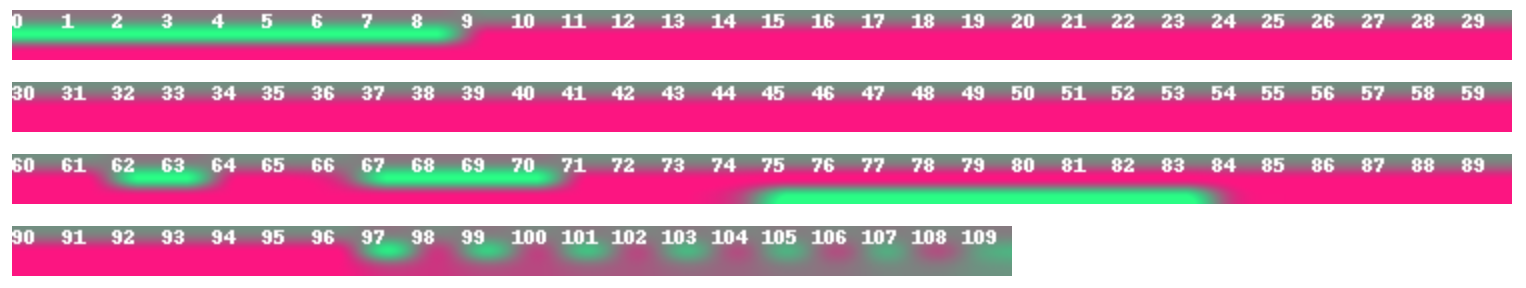
\includegraphics[width=\textwidth]{images/classifier/neuron-activations-simple-rnn-model-3/flack-55-martin}\\
%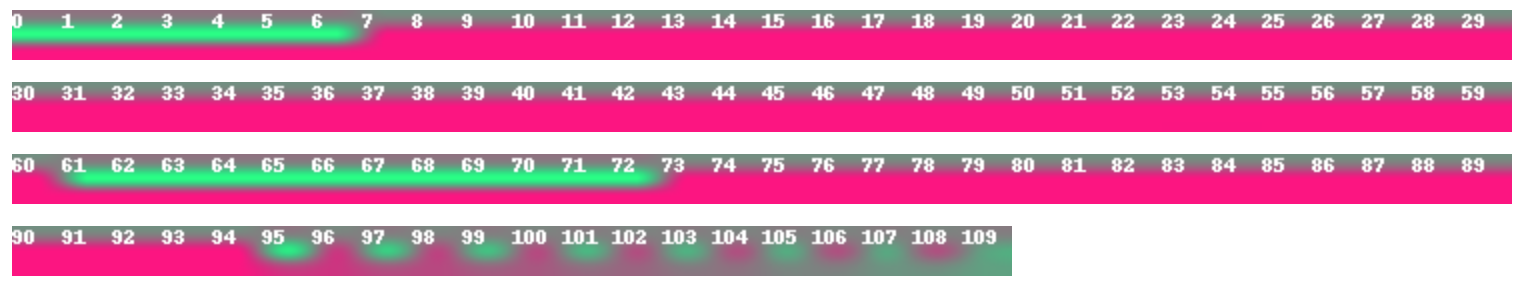
\includegraphics[width=\textwidth]{images/classifier/neuron-activations-simple-rnn-model-3/flack-59-martin}\\
%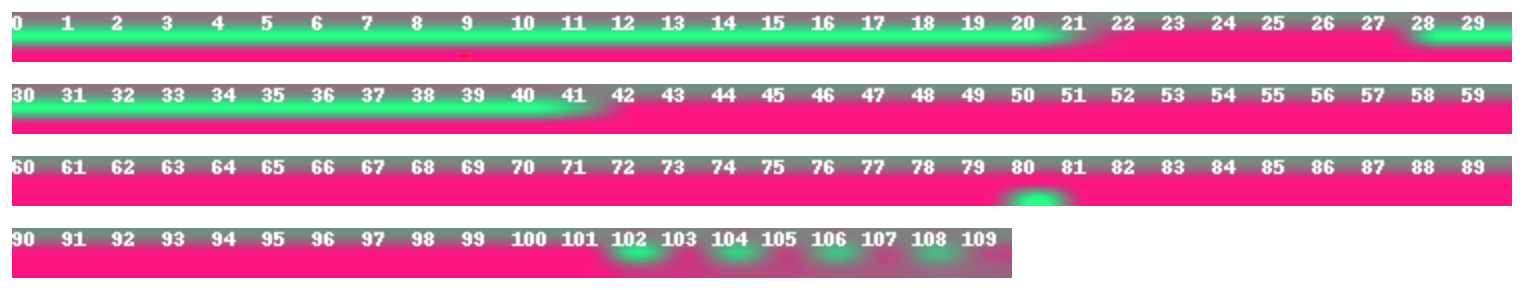
\includegraphics[width=\textwidth]{images/classifier/neuron-activations-simple-rnn-model-3/flack-68-rasmus}\\
\end{tabular}
    \caption{Simple RNN neuron activations for back handspring samples}
    \label{back-handspring-neuron-activations-simple-rnn}
\end{figure*}










